
\section{Explosion filtering, EXFILTER} 
\label{sect:exfilter}

\index{Explosion filtering}\index{EXFILTER}\index{Catalog work} The program EXFILTER is used to identify probable explosions in a catalog of seismic events. Man-made seismic events like quarry blasts, mining explosions and other explosions show a certain distribution in time and space. Therefore the method of explosion identification here is based on normalizing the time of day distribution of seismic event occurrence as a function of area. The program works on the following principle: Areas where explosions occur are defined. If an event is located in one of these areas, with a magnitude below a given maximum magnitude, with a depth less than a given maximum depth, within a given time of day interval and within a given year interval, it is identified and marked as probable explosion. The areas are defined by \index{Polygon}polygons of any shape. For definition of the filter areas, a list of mine locations (with consideration of location accuracy), locations of explosions and locations of event clusters (they might be clearly related to mine locations, but others might indicate unknown explosion sites) can be used. The next step is to define the parameters for each area to get a normal time of day distribution. They can be determined following the steps: 

\begin{itemize}
\item[1)]
\begin{itemize}
\item[]
- get the time of day distribution of events (program CATSTAT) 
\item[]
- select a time window of probable explosions 
\item[]
- select events within time window of probable explosions 
\end{itemize}
\item[2)]
\begin{itemize}
\item[]
- get the distribution of magnitudes of events within time window of probable explosions (program BVALUE) 
\item[]
- select the maximum magnitude 
\end{itemize}
\item[3)]
\begin{itemize}
\item[]
- test parameters defined with program EXFILTER for the defined area and adjust the parameters if the time of day distribution is not normal. 
\end{itemize}
\end{itemize}

For more details, see \citet{ottemoller1995}.

The program uses a parameter file, \texttt{EXFILTER.PAR} which MUST be located in the DAT directory. 

An example of the parameter file \texttt{EXFILTER.PAR}

\verbatiminput{include/exfilter.par}

The EXFILTER program searches for probable explosions using a 
catalog-file as input and marks events that might be explosions with 
'P' as Event ID in the output file \texttt{exfilter.out}. 
Example of program run 

\begin{verbatim}
<exfilter> 

NUMBER OF AREAS: 55 

 FILENAME... ? 
june.cat
 ************************************
 Number of probable explosions found: 90
 Output written in file: exfilter.out
 ************************************ 
\end{verbatim}

\begin{figure}
\htmlimage{scale=2.0}
\centerline{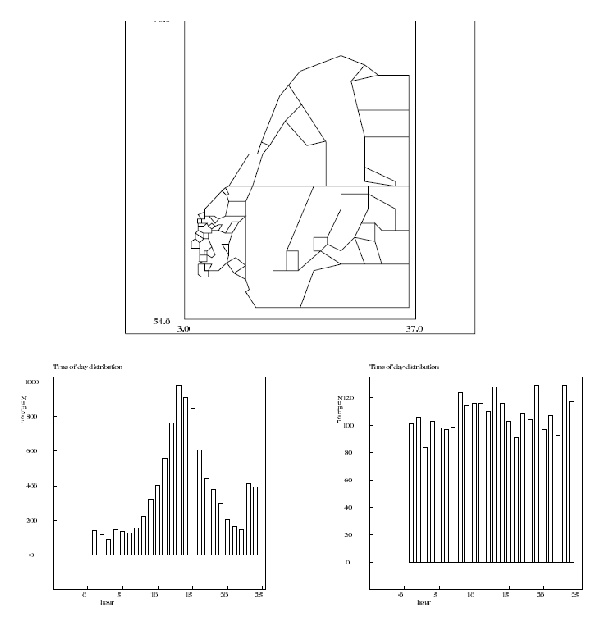
\includegraphics[width=0.9\linewidth]{fig/fig45}}
\caption{Figures that show how the exfilter works for events in Scandinavia:\newline
The top figure shows the filter areas used for Scandinavia. The bottom right figure shows the time of day distribution for a 10 year Scandinavian catalog before filtering (made with CATSTAT) and the figure bottom left shows the distribution after filtering.}
\label{fig:exfilter}
\end{figure}


